\documentclass[11pt, titlepage]{article}

\usepackage{times,fullpage,graphicx,amsmath, cite, alltt, enumitem, titlesec, verbatim, array}
\usepackage[pdfborder={0 0 0}]{hyperref}
\usepackage{lipsum}
\newcounter{question}
\setcounter{question}{0}

\usepackage{subfigure}

\newcommand\Que[1]{%
   \leavevmode\par
   \stepcounter{question}
   \noindent
   \thequestion. Q --- #1\par}

\newcommand\Ans[1]{%
    \leavevmode\par\noindent
   {\leftskip37pt
    A. --- #1 \par }}


\newcommand{\supth}{{\mathrm{th}}}


\titleformat*{\paragraph}{\large\bfseries}


\title{The Preseq Manual}
\author{Timothy Daley \and Victoria Helus \and Andrew Smith }

\begin{document}
\maketitle

\tableofcontents

\newpage

\section{Quick Start}
\label{chap:quickstart}
\newcommand{\fn}[1]{\texttt{#1}}



The \textbf{preseq} package is aimed at predicting
the yield of distinct reads from a genomic library
from an initial sequencing experiment.  The estimates
can then be used to examine the utility of further
sequencing, optimize the sequencing depth,
or to screen multiple libraries to avoid low complexity
samples.~\\[-.2cm]

\noindent The two main programs are \fn{c\_curve} and \fn{lc\_extrap}.
\fn{c\_curve} samples reads without replacement from the 
given mapped sequenced read file or duplicate count file to estimate the yield
of the experiment and the subsampled experiments.  These estimates
are used construct the complexity
curve of the experiment.  \fn{lc\_extrap} uses rational function approximations
of Good \& Toulmin's~\cite{good1956number} non-parametric
empirical Bayes estimator to predict the yield
of future experiments, in essence looking into the future
for hypothetical experiments.  \fn{lc\_extrap} is used to predict 
the yield and then \fn{c\_curve} can be used to check the yield
from the larger experiment.

\newpage

\section{Installation}
\label{sec:install}

\paragraph{Download}
\label{sub:download}~\\~\\[-.2cm]
\raggedright{\textbf{preseq} is available at }
\url{http://smithlab.cmb.usc.edu/software/}.


\paragraph{System Requirements}
\label{sub:require}
~\\~\\[-.2cm]
\textbf{preseq} runs on Unix-type system
with GNU Scientific Library (GSL), available
at ~\url{http://www.gnu.org/software/gsl/}.  
If the input file is in BAM format, BamTools is
required, available at ~\url{https://github.com/pezmaster31/bamtools}.
If the input is 
a text file of counts in a single column or is 
in BED format, 
BamTools is not required.
It has been tested on Linux and 
Mac OS-X.  

\paragraph{Installation}~\\~\\[-.2cm]
\label{sub:install}
Download the source code and decompress
it with 
\begingroup \fontsize{9pt}{12pt}\selectfont \begin{alltt}
 $ tar -jxvf preseq.tar.bz2
\end{alltt} \endgroup
% 
Enter the \textbf{preseq/} directory and run
\begingroup \fontsize{9pt}{12pt}\selectfont \begin{alltt}
$ make all
\end{alltt}\endgroup

The input file may possibly be in BAM format. If the root directory 
of BamTools is \$bamtools, instead run
\begingroup \fontsize{9pt}{12pt}\selectfont \begin{alltt}
$ make all BAMTOOLS_ROOT=$bamtools
\end{alltt}\endgroup
Output after typing this command should include the flag \fn{-DHAVE\_BAMTOOLS} if the linking is successful. If compiled successfully, the executable files are available
in \textbf{preseq/}. 

If a BAM file is used as input without first having run \begingroup \fontsize{9pt}{11pt}\selectfont  \fn{\$ make all BAMTOOLS\_ROOT=/loc/of/bamtools}\endgroup, then the following error will occur: \begingroup \fontsize{9pt}{12pt}\selectfont \fn{terminate called after throwing an instance of 'std::string'}\endgroup. 

\newpage

\section{Using preseq}
\label{sec:usage}

\paragraph{Basic usage}~\\~\\[-.2cm]
\label{sub:basic}
To generate the complexity plot of a genomic
library from a read file in BED or BAM format or a duplicate count file,
use the program \fn{c\_curve}.  Use
\fn{-o} to specify the output name.
\begingroup \fontsize{9pt}{12pt}\selectfont \begin{alltt}
$ ./c_curve -o complexity_output.txt input.bed
\end{alltt}\endgroup

To estimate the future yield 
of a genomic library
using an initial experiment in BED  format,
use the program \fn{lc\_extrap}.
The required options are \fn{-o} to specify
the output of the yield estimates and 
the input file, which is either a BED
file sorted by chromosome, end position, start
position, and strand or a BAM file
sorted with BamTools or SAMTools sort function. Additional 
options are available and are detailed below. 
\begingroup \fontsize{9pt}{12pt}\selectfont 
\begin{alltt}
$ ./lc_extrap -o future_yield.txt input.txt 
\end{alltt}\endgroup

\newpage

\section{File Format}
\label{sec:format}

\paragraph{Sorted read files in BED or BAM format}~\\~\\[-.2cm]
Input files are sorted mapped read files in BED or BAM format,
or a text file consisting of one column giving the observed read counts.
The 
programs require that BED files are sorted by chromosome, 
end position, start position, and strand.  This can be achieved
by using the command line function sort as follows: 
\begingroup \fontsize{9pt}{12pt}\selectfont \begin{alltt}
sort -k 1,1 -k 2,2n -k 3,3n -k 6,6 input.bed > input.sort.bed
\end{alltt}\endgroup
BAM format read files should be sorted by chromosome and
start position.  This can be done with either SAMTools (available at
~\url{http://samtools.sourceforge.net/} ) or BamTools
sort functions. If the input is in BAM format, then the flag
\fn{-B} must be included.  

If the input is paired end, the option \fn{-P} can be set.
In this case only concordantly mapped reads are counted.
This means that if either end does not map or if
the mapping locations of the two ends are not compatible, the read
is not counted.  If a large number of reads are disconcordant, then
the default single end should be used.  In this case only the mapping 
location of the first mate
is used as the unique molecular identifier~\cite{kivioja2011counting}.



\paragraph{Text files of observed read counts}~\\~\\[-.2cm]
For more general applications \textbf{preseq} allows the input
to be a text file of observed read counts, one count per
line.   To specify this input, the option \fn{-V} must be set.

Such a text file can typically be constructed by command 
line arguments.  Take for example an unmapped sequencing
experiment in FASTQ format.  To predict the complexity, the unique
molecular identifier needs to use only the observed sequence.
For instance, a unique molecular identifier used may be the first
20 bases in the observed sequence.  A command line argument
to construct the counts would then be
\begingroup \fontsize{9pt}{12pt}\selectfont \begin{alltt}
awk '{if (NR%4==2) print substr($0,1,20);}' input.fastq | sort | uniq -c 
\end{alltt}\endgroup
\begingroup \fontsize{9pt}{12pt}\selectfont \begin{alltt}| awk '{print $1}' > counts.txt
\end{alltt}\endgroup
More complicated unique molecular identifiers
can be used, such as mapping position plus a random barcode,
but are too complicated to detail in this manual. For questions with such usage, please contact us at \href{mailto:tdaley@usc.edu}{\nolinkurl{tdaley@usc.edu}}

\newpage

\section{Detailed usage}
\label{chap:detail}

\paragraph{c\_curve}~\\~\\[-.2cm]
\label{sec:complexityplot}

\fn{c\_curve} is used to compute the 
expected complexity curve of a mapped read file by 
subsampling smaller experiments without replacement 
and counting the distinct reads.
Output is a text file with two 
columns.  The first gives the total number
of reads and the second the corresponding number
of distinct reads.

\begin{description}[style=multiline,leftmargin=6cm,font=\ttfamily]
\item[\begingroup \fontsize{9pt}{12pt}\selectfont-o, -output\endgroup] Name of output file. Default prints to screen
\item[\begingroup \fontsize{9pt}{12pt}\selectfont-v -verbose\endgroup] Prints more information
\item[\begingroup \fontsize{9pt}{12pt}\selectfont-s, -step\endgroup] The step size for samples. Default is 1 million reads
\item[\begingroup \fontsize{9pt}{12pt}\selectfont-B, -bam\endgroup] Input file is in BAM format
\item[\begingroup \fontsize{9pt}{12pt}\selectfont-P, -pe\endgroup] Input is a paired end read file
\item[\begingroup \fontsize{9pt}{12pt}\selectfont-H, -hist\endgroup] Input is a text file of the observed histogram
\item[\begingroup \fontsize{9pt}{12pt}\selectfont-V, -vals\endgroup] Input is a text file of read counts
\end{description}

\paragraph{lc\_extrap}~\\~\\[-.2cm]
\label{sec:librarycomplexity}

\fn{lc\_extrap} is used to generate
the expected yield for theoretical larger
experiments and bounds on the number of distinct 
reads in the library and the associated confidence
intervals, which is computed by bootstrapping the observed duplicate count histogram.
Output is a text file with four columns.  The
first is the total number of reads, second
gives the corresponding average
expected number of distinct reads, and the 
third and fourth give the lower and
upper
limits of the confidence interval.
Specifying verbose will print out the histogram
of the input file.  


\begin{description}[style=multiline,leftmargin=6cm,font=\ttfamily]
\item[\begingroup \fontsize{9pt}{12pt}\selectfont-o, -output\endgroup] Name of output file. Default prints to screen
\item[\begingroup \fontsize{9pt}{12pt}\selectfont-e, -extrapolation\_length \endgroup]The maximum number of total reads to compute yield estimates for.  The default is 10 billion reads.
\item[\begingroup \fontsize{9pt}{12pt}\selectfont-v, -verbose\endgroup] Prints more information
\item[\begingroup \fontsize{9pt}{12pt}\selectfont-s, -step\endgroup] The step size between yield estimates. Default is 1 million reads
\item[\begingroup \fontsize{9pt}{12pt}\selectfont-b, -bootstraps\endgroup] The number of bootstraps used to compute the confidence intervals. Default is 100
\item[\begingroup \fontsize{9pt}{12pt}\selectfont-c, -cval\endgroup] Level for confidence intervals.  Default is 0.95
\item[\begingroup \fontsize{9pt}{12pt}\selectfont-B, -bam\endgroup] Input file is in BAM format
\item[\begingroup \fontsize{9pt}{12pt}\selectfont-P, -pe\endgroup] Input is a paired end read file
\item[\begingroup \fontsize{9pt}{12pt}\selectfont-H, -hist\endgroup] Input is a text file of the observed histogram
\item[\begingroup \fontsize{9pt}{12pt}\selectfont-V, -vals\endgroup] Input is a text file of read counts
\item[\begingroup \fontsize{9pt}{12pt}\selectfont-Q\endgroup] Computes the expected yield without confidence intervals and avoids bootstrapping for significantly faster computations 
\end{description}

\newpage

\section{lc\_extrap Examples}
\label{sec:examples}

Usage and output of \fn{c\_curve} is similar, so the following examples are of \fn{lc\_extrap} and its different options. 


\paragraph{Using a sorted read file in BED (or BAM with the \fn{-B} flag) format as input}~\\
\begingroup \fontsize{9pt}{12pt}\selectfont \begin{alltt}
$ ./lc_extrap -o future_yield.txt input.bed
\end{alltt}\endgroup

\begin{table}[ht!]
 \fontfamily{pcr}\fontsize{9pt}{12pt}\selectfont
\begin{tabular}{llll}

TOTAL\_READS &  EXPECTED\_DISTINCT  & LOGNORMAL\_LOWER\_95\%CI  & LOGNORMAL\_UPPER\_95\%CI \\ \hline
0 & 0 & 0 & 0\\
1000000.0 & 955978.6 & 953946.4 & 958015.1\\
2000000.0 & 1897632.0 & 1892888.4 & 1902387.5\\
3000000.0 & 2829410.5 & 2819146.4 & 2839712.0\\
4000000.0 & 3751924.0 & 3732334.5 & 3771616.2\\
. & . & . & .\\
. & . & . & .\\
. & . & . & .\\
. & . & . & .\\
9999000000.0 & 185394069.4 & 76262245.8 & 450694319.0\\
\end{tabular}
\end{table}



This example uses a sorted read file in BED format from an initial experiment generated from single sperm cells. 
As noted above, the default step size between yield estimates is 1 million, the default confidence interval level is 95\%, and the default extrapolation length is 10 billion. 

\paragraph{Using a sorted read file in BED format as input, including the verbose option}~\\
\begingroup \fontsize{9pt}{12pt}\selectfont \begin{alltt}
$ ./lc_extrap -o future_yield.txt input.bed -v
\end{alltt}\endgroup

As \fn{lc\_extrap} is running, information will print to screen that gives a read counts histogram of the input file which truncates after the first bin value that has zero observations. Included here is the first 10 lines of what would be observed: 


\begingroup \fontsize{9pt}{12pt}\selectfont \begin{alltt}
TOTAL READS     = 536855
DISTINCT READS  = 516200
DISTINCT COUNTS = 48
MAX COUNT       = 269
COUNTS OF 1     = 511413
MAX TERMS       = 100
OBSERVED COUNTS (270)
1       511413
2       2202
3       597
\end{alltt}\endgroup



\paragraph{Using a sorted read file in BED format as input, with options}~\\
\begingroup \fontsize{9pt}{10pt}\selectfont \begin{alltt}
$ ./lc_extrap -e 15000000 -s 500000 -b 90 -c .90 -o future_yield.txt input.bed 
\end{alltt}\endgroup
\newpage

\begin{table}[ht!]
 \fontfamily{pcr}\fontsize{9pt}{12pt}\selectfont
\begin{tabular}{llll}
TOTAL\_READS & EXPECTED\_DISTINCT & LOGNORMAL\_LOWER\_90\%CI & LOGNORMAL\_UPPER\_90\%CI \\ \hline
0 & 0 & 0 & 0 \\
500000.0 & 481098.5 & 480329.1 & 481869.1 \\
1000000.0 & 956070.6 & 954493.7 & 957650.2 \\
1500000.0 & 1428183.4 & 1425461.7 & 1430910.2 \\
2000000.0 & 1897886.0 & 1892501.7 & 1903285.7 \\
. & . & . & .\\
. & . & . & .\\
. & . & . & .\\
. & . & . & .\\
14500000.0 & 12932529.0 & 12056525.8 & 13872180.9\\
\end{tabular}
\end{table}

Notice the slight changes, with the step sizes of the extrapolation now at 500,000 as specified, and the maximum extrapolations ending at 15,000,000. The confidence intervals are now at a level of 90\%. 

\paragraph{Using a histogram or read counts as input}~\\~\\[-.2cm]

\fn{lc\_extrap} allows the input file to be an observed histogram. An example of the format of this histogram is as followed:
\begingroup \fontsize{9pt}{12pt}\selectfont \begin{alltt}
1       1.68166e+07
2       4.55019e+06
3       1.93787e+06
4       1.07257e+06
5       708034
6       513134
7       384077
8       282560
9       206108
10      146334
\end{alltt}\endgroup

The following command will give output of the same format as the above examples.\begingroup \fontsize{9pt}{12pt}\selectfont \begin{alltt} $./lc_extrap -o future_yield.txt -H histogram.txt \end{alltt}\endgroup

Similarly, both \fn{lc\_extrap} and \fn{c\_curve} allow the option to input read counts, which is just the histogram but with the bin values excluded (text file should contain ONLY the observed counts in a single column). Command should be run with the \fn{-V} flag: \begingroup \fontsize{9pt}{12pt}\selectfont \begin{alltt} $./lc_extrap -o future_yield.txt -V counts.txt \end{alltt}\endgroup

\newpage

\section{preseq application examples}

\subsection*{Screening multiple libraries}
\label{sec:multlib}
This section provides a more detailed example using data from different experiments to illustrate how preseq might be applied. Because it is important to avoid spending time on low complexity samples, it is important to decide after observing an initial experiment whether or not it is beneficial to continue with sequencing. The data in this example comes from a study (accession number SRA061610) using single cell sperm cells amplified by Multiple Annealing and Looping Based Amplification Cycles (MALBAC)~\cite{lu2012probing} and focuses on three libraries coming from different experiments from the study (SRX205369, SRX205370, SRX205372). 

These libraries help show what would be considered a relatively poor library and a relatively good library, as well as compare the complexity curves obtained from running \fn{c\_curve} and \fn{lc\_extrap}, to show how \fn{lc\_extrap} would help in the decision to sequence further. The black diagonal line represents an ideal library, in which every read is a distinct read (though this cannot be achieved in reality). The full experiments were down sampled at 5\% to obtain a mock initial experiment of the libraries, as shown here, where we have the complexity curves  of the initial experiments generated by \fn{c\_curve}:
~\newline
\newline
\begin{figure}[h!]
\centering
\centering{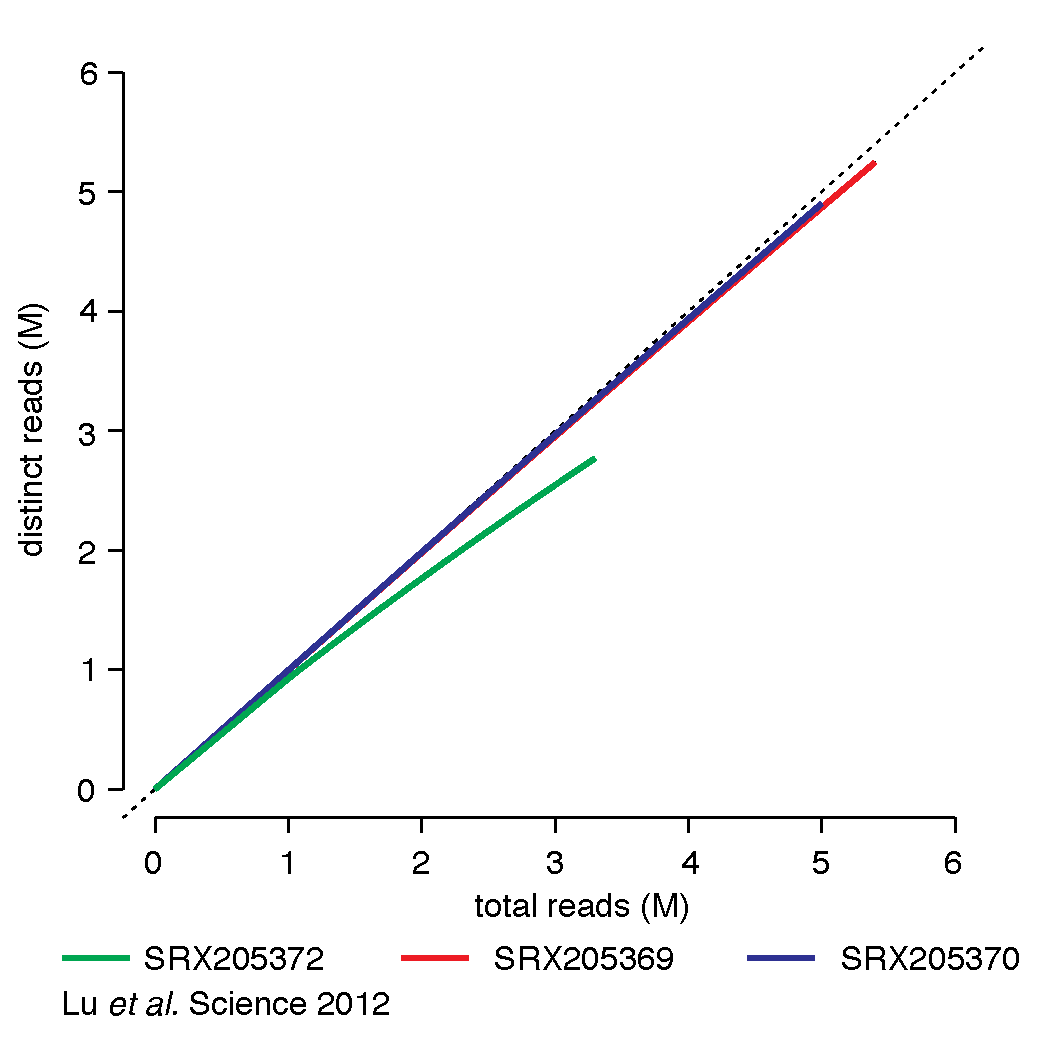
\includegraphics[totalheight = 0.5\textheight, trim=0cm 0cm 0cm 2cm, clip = true]{InitialExperimentComplexityCurves_copy.pdf}}
\caption{Initial observed complexities}
\end{figure}

With such a relatively small amount of reads sequenced, it is hard in the first stages of a study to guess at whether it is not worth sequencing a library further, as all three libraries seem to be relatively good. 

This is a comparison of the full experiment complexity curves and the extrapolated complexity curves created using information from the initial experiments above as input. The dashed lines indicate the complexity curves predicted by \fn{lc\_extrap}, and the solid lines are the expected complexity curves of the full experiments, obtained using \fn{c\_curve}. Note that the dashed curves follow the solid curves very closely, only differing slightly towards the end, meaning \fn{lc\_extrap} gives a good predicted yield curve.  Using this, it is clear that if the initial experiments were the only available data and \fn{lc\_extrap} was run, SRX205372 would likely be discarded, as it is a poor library, and SRX205369 and SRX205370 would probably be used for further sequencing, as their complexity curves indicate that sequencing more would yield enough information to justify the costs.  If the researcher were to only want to sequence one library deep, then SRX205370 would be an obvious choice. 
\newline
\newline
\begin{figure}[h!]
\centering
\centering{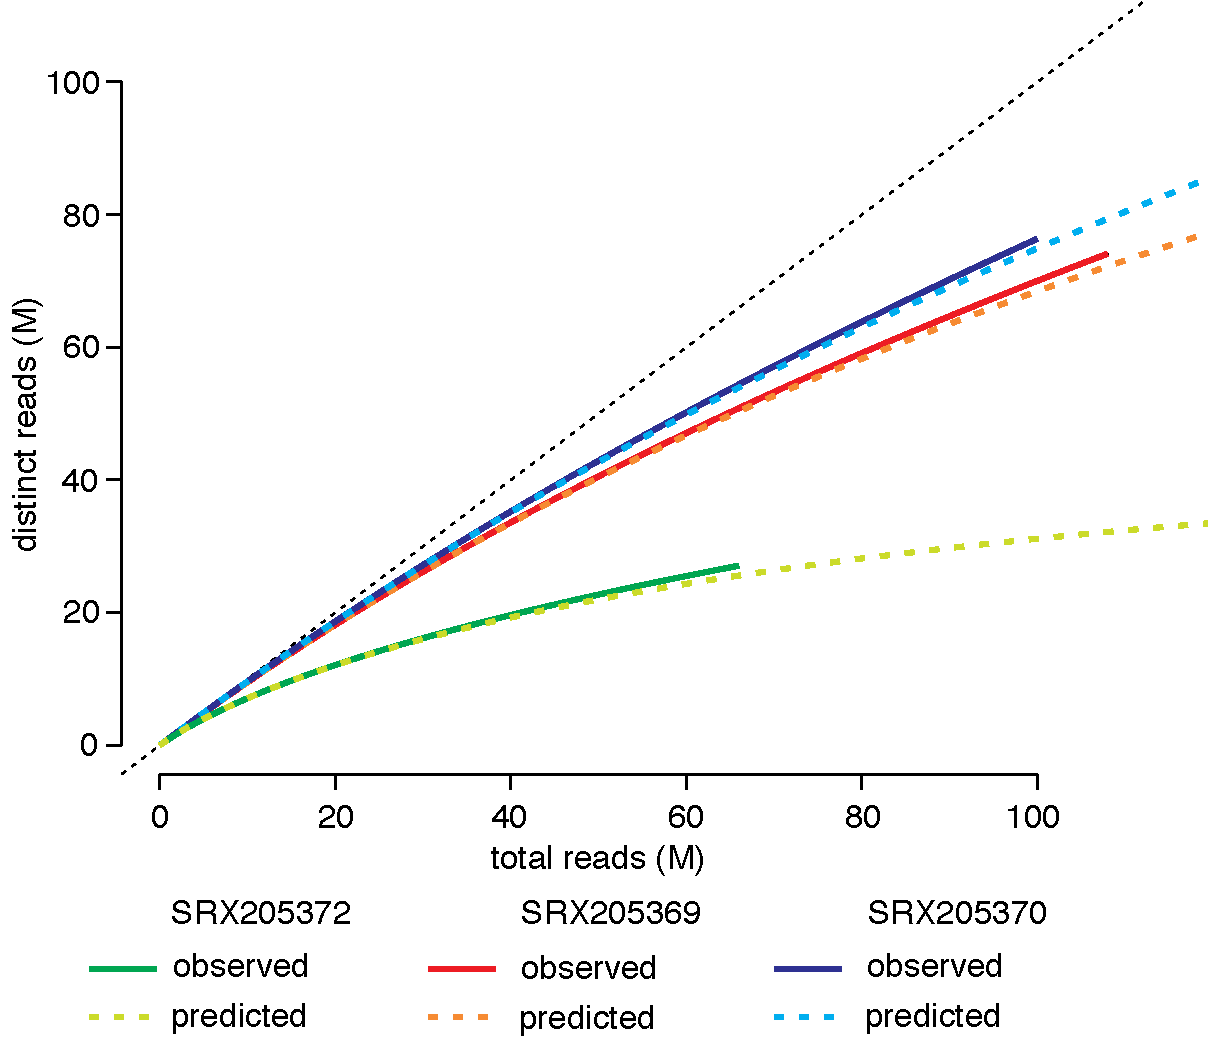
\includegraphics[totalheight = 0.5\textheight, trim=0cm 0cm 0cm 2cm, clip = true]{FullExperiment_copy.pdf}}
\caption{Estimated versus observed library complexities.}
\end{figure}


\newpage


\subsection*{Saturation of reads and junctions for RNA sequencing experiments}

A recent paper from the Rinn lab~\cite{mercer2011targeted}
developed a targeted capture RNA sequencing
protocol to deeply investigate chosen portions of the transcriptome.  
A comparison of the results from a standard RNA sequencing
experiment (RNA-seq; SRA accession SRX061769) and a targeted capture RNA sequencing
experiment (Capture-seq; SRA accession SRX061768) reveals
a startling amount of transcriptional complexity missed by standard
RNA sequencing in the targeted regions.  A large number of
rare transcriptional events such as alternative splices, alternative isoforms,
and long non-coding RNAs were newly identified with the targeted sequencing.

A current vigorous debate exists on whether these rare events are truly transcriptional
events or are merely due to sequencing or transcriptional noise 
(see~\cite{van2010most} and~\cite{clark2011reality}).  We do not seek to address
these issues, but merely to comment on the true complexity
of rare transcriptional events in sequencing libraries identified by current
protocols.

We took the two Illumina sequencing libraries from~\cite{mercer2011targeted} and
mapped them according to the protocol given.  We downsampled $10 \%$ of the library
and compared the estimated library complexities (single end) with the observed library
complexity for both libraries.  We also took the junction information contained in the file
junctions.bed in the Tophat output folder to estimate the junction complexity.  Since
the 5th column (excluding the first line) is the number of times each
distinct junction is observed, we can simply cut out these values as input for
\fn{lc\_extrap} or \fn{c\_curve} with the flag \fn{-V}.  A simple command line example follows.

\begin{verbatim}
sed '1d' tophat/junctions.bed | cut -f 5  > junction_vals.txt
~/preseq/lc_extrap -V -o junction_vals_extrap.txt junction_vals.txt
\end{verbatim}

The output \fn{TOTAL\_READS} column will be in terms of the number of 
total junctions (not reads), so scaling by the average number of junctions per 
read will give the appropriate scale for plotting on the x-axis.  

\begin{figure}[h!]
\centering{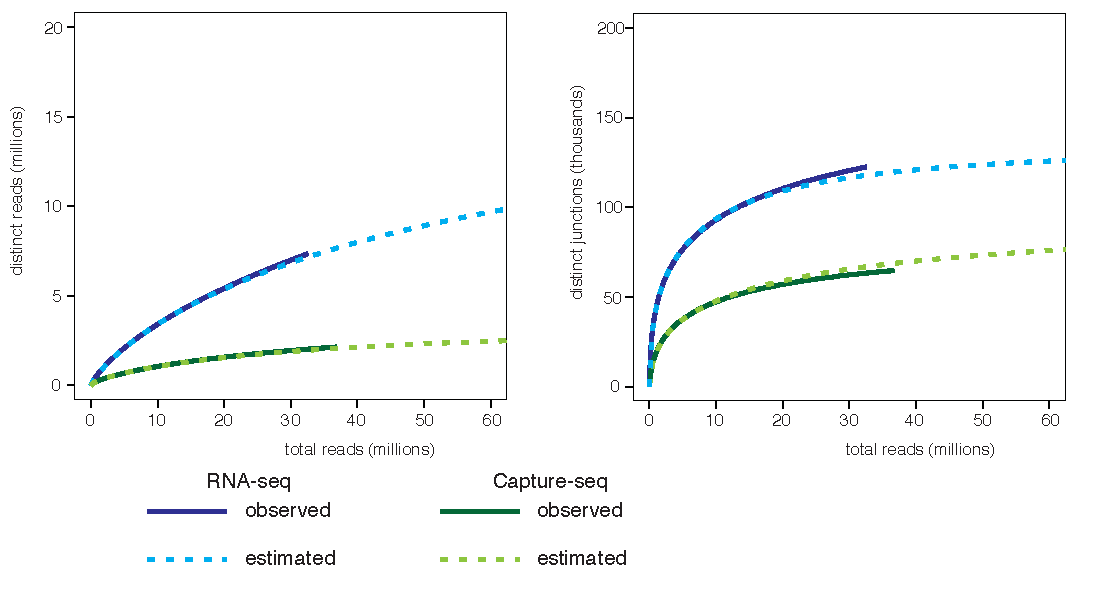
\includegraphics[width=14cm]{compare_RNA_Capture_junction_complexity.pdf}}
\caption{A comparison of complexities of standard RNA-seq and 
targeted capture RNA-seq.  Estimated complexities for both cases were 
estimated using 10\% of the data.}
\end{figure}

We see from the estimated library that the RNA-seq library is far
from saturated, while it appears that the Capture-seq library
may be close.  On the other hand, the junction complexity of
both libraries indicates that the full scope of juctions identified
by Tophat is far from saturated in both libraries.  This indicates
that large number of rare junctions still remain to be identified
in the libraries.


\newpage


\section{FAQ}

\Que{I compile the preseq binaries but receive the error 

\fn{terminate called after throwing an instance of 'std::string'}
}

\Ans{This error is typically called because either the flag -B was not included to 
specify bam input or because the linking to bamtools was not included when
compiling preseq.  To ensure that the linking was done properly, check for the flag
\fn{-DHAVE\_BAMTOOLS}.}

\Que{I receive the error 

\fn{ERROR:  too many iterations, poor sample}

when running \fn{lc\_extrap}
}

\Ans{
There are a number of causes for this.  Most commonly this is due to the presence of
defects in the approximation which cause the estimates to be unstable.  Setting the step
size larger (with the flag \fn{-s}) will help to avoid the defects.  The default step size is 1M reads or
0.05\% of the input sample size rounded up to the nearest million, whichever is larger.  
A consequence of this action will be a reduction in the observed smoothness of the curve.
}


\Que{When running \fn{lc\_extrap}, I receive the error 

\fn{sample not sufficiently deep or duplicates removed}
}

\Ans{There may be two causes for this, either duplicates have been removed and 
every observed read is distinct or there is not sufficient variation in the library for 
\fn{lc\_extrap} to run.

The information required by \fn{lc\_extrap} is essentially the number of times each
distinct read was observed, which we call the duplicate counts.  
Without sufficient variation in the duplicate counts we cannot extrapolate the 
complexity of the library.  We have set the minimum require max duplicate count
(the largest number of times any read has been observed) to 5.  
If the input library does not satisfy this, then either a parametric model such
as a Poisson or Negative Binomial may be appropriate or deeper
sequencing may be required.}

\vspace{5mm}
Any other questions can be sent to \href{mailto:tdaley@usc.edu}{\nolinkurl{tdaley@usc.edu}}.
The preseq software is still under development so we would appreciate any 
advice or comments. Thanks!

\newpage

\bibliographystyle{plain}
\bibliography{biblio}





\end{document}